% !TEX root = ../Coherence.tex


%%%%%%%%%%%%%%%%%%%%%%%%%%%%%%%%%%%%%

\subsection{Symmetric monoidal categories} 

We now formulate Mac Lane's coherence theorem for \emph{symmetric} monoidal categories in the same style as above. We construct the free symmetric monoidal category on a set $S$.
We define a small category $\mathcal{S}^{\mathrm{ML}}$ whose set ${\cal T}_S$  is  given by the following rules:
\begin{enumerate}
    \item if $a \in S$, then $a\in{\cal T}_S$;
    \item if $t_1 \in {\cal T}_S$ and $t_2 \in {\cal T}_S$, then $t_1 \otimes t_2\in{\cal T}_S$.
\end{enumerate}
We call the elements of $S$ generating objects.

Now we define a set $M^{\mathrm{ML}}$ of basic morphisms $\beta: (t_1 \otimes t_2) \otimes t_3 \leftrightarrow t_1 \otimes (t_2\otimes t_3) : \beta^{-1}$  and $\tau: t_1\otimes t_2 \leftrightarrow t_2 \otimes t_1 : \tau^{-1}$,  for every $t_1,t_2,t_3  \in {\cal T}_S$
.
We then define the generating morphisms of  $\mathcal{S}^{\mathrm{ML}}$ by the following rules:
\begin{enumerate}
    \item if $\phi \in M^{\mathrm{ML}}$, then $\phi$ is a generating morphism; 
    \item if $\phi : t_1 \to t_2$ is a generating morphism and $t_3 \in {\cal T}_S$, then $\phi \otimes \id : t_1 \otimes t_3 \to t_2 \otimes t_3$ and $\id \otimes \phi : t_3 \circ_j t_1 \to t_3 \otimes t_2$ are generating morphisms.
\end{enumerate}
We then define $\mathcal{S}^{\mathrm{ML}}$ as the free category over all generating morphisms. 
This finishes the construction of the category $\mathcal{S}^{\mathrm{ML}}$.

\begin{definition}
    We denote  by $\mathcal{F}(S)$ the quotient of $\mathcal{S}^{\mathrm{ML}}$ by localization (inverting the $\beta$ and $\tau$ morphisms), the axioms of bifunctors, the naturality conditions for $\beta$ and $\tau$, the coherence diagrams defining a  symmetric monoidal categories, i.e;. the pentagons and Mac Lane's hexagons.
    \end{definition}

We obtain that $\mathcal{F}(S)$ is the free  symmetric monoidal category on $S$. 
That is, for any symmetric monoidal category $\mathcal{C}$, and for any function $\rho : S \to \obj(\mathcal{C})$, there is a unique \emph{strict} morphism of symmetric monoidal categories $\mathcal{F}(S) \to \mathcal{P}$ which extends $\rho$. It sends the formal basic morphisms to the actual canonical morphisms of $\mathcal{C}$.
By precomposing it with the quotient map $[-]:\mathcal{S} \to \mathcal{F}(S)$, we get  functor $\ll\!-\!\gg^{\mathrm{ML}}:\mathcal{S}^{\mathrm{ML}} \to \mathcal{C}$.

\smallskip
It turns out that Kapranov's topological proof is not based on the above presentation of $\mathcal{F}(S)$, but implicitly on another presentation of this category, that is made explicit in~\cite{baralicSimplePermutoassociahedron2019}. 
We recall this presentation. We define another category $\mathcal{S}^{\mathrm{K}}$ as follows. Its objects are the same as those of $\mathcal{S}^{\mathrm{ML}}$. We define a set $M^{\mathrm{K}}$ of basic morphisms $\beta: (t_1 \otimes t_2) \otimes t_3 \leftrightarrow t_1 \otimes (t_2\otimes t_3) : \beta^{-1}$ for every $t_1,t_2,t_3  \in {\cal T}_S$ , and $\tau: \mu_1\otimes \mu_2 \leftrightarrow \mu_2 \otimes \mu_1 : \tau^{-1}$ for every $\mu,\nu  \in S$, i.e., we limit $\tau$ to generating objects.
Generating morphisms are defined in the same way as for $\mathcal{S}^{\mathrm{ML}}$.
We not that by construction $\mathcal{S}^{\mathrm{K}}$ is a wide subcategory of $\mathcal{S}^{\mathrm{ML}}$

\begin{definition}
    We denote   by $\mathcal{F}(S)^{\mathrm{K}}$ the quotient of $\mathcal{S}^{\mathrm{K}}$ by localization (inverting the $\beta$ and $\tau$ morphisms), the axioms of bifunctors, the naturality conditions for $\beta$, the coherence diagrams defining a  monoidal categories (i.e. the pentagons above) and by the following axiom in dodecagonal form.
\end{definition}
Let $\mathcal{C}$  be a symmetric monoidal category. Then by freeness  $\rho : S \to \obj(\mathcal{C})$, $\rho$ extends uniquely to a functor $\ll\!-\!\gg^{\mathrm{K}}:\mathcal{S}^{\mathrm{K}} \to \mathcal{C}$.
This functor is the restriction of $\ll\!-\!\gg^{\mathrm{ML}}$ to $\ll\!-\!\gg^{\mathrm{K}}$



\begin{proposition}
\label{thm:coherence-Kapranov}
    For any symmetric monoidal category $\mathcal{C}$, for any  function $\rho : S \to \obj(\mathcal{C})$, and for any two parallel morphisms $\phi_1,\phi_2: t_1 \to t_2$ in~$\mathcal{S}^{\mathrm{K}}$, we have $\ll\!\phi_1\!\gg^{\mathrm{K}}=\ll\!\phi_2\!\gg^{\mathrm{K}}$.
\end{proposition}
\begin{proof}
The conclusion will readily follow from the following two properties
\begin{enumerate}
\item If $\phi_1,\phi_2: t_1 \to t_2$ in~$\mathcal{S}^{\mathrm{K}}$, then $[\phi_1]^{\mathrm{K}}=[\phi_2]^{\mathrm{K}}$, where $[-]^{\mathrm{K}}:\mathcal{S}^{\mathrm{K}}\to  \mathcal{F}(S)^{\mathrm{K}}$ is the quotient functor.  
\item The relations in Kapranov presentation are valid in $\mathcal C$.
\end{enumerate} 
Indeed, (2) says that $\ll\!-\!\gg^{\mathrm{K}}$ factors through $[-]^{\mathrm{K}}$, hence the statement is reduced to proving (1).

{\color{blue} Pour prouver (1) géométriquement, il faut exhiber la correspondance entre objets et 0-faces etc. comme pour les opéraèdres, dans le polytope de Ziegler et al. Pour prouver (2), on montre comment prouver les relations de Kapranov à partir des relations de Mac Lane = le dodécagone comme deux hexagones plus une naturalité}
\end{proof}

\begin{proposition} \label{Kapranov-MacLane}
The identity-on-objects  functor from  $\mathcal{F}(S)^{\mathrm{K}}$ to 
$\mathcal{F}(S)$ that maps $[\phi_1]^{\mathrm{K}}$ to $[\phi_1]$ is an isomorphism of categories.
\end{proposition}

\begin{proof}
TO DO (on utilise \cref{thm:coherence-Kapranov}!).
\end{proof}

\begin{thm}[Coherence theorem]
\label{thm:coherence-MacLane}
    For any symmetric monoidal category $\mathcal{C}$, for any  function $\rho : S \to \obj(\mathcal{C})$, and for any two parallel morphisms $\phi_1,\phi_2: t_1 \to t_2$ in~$\mathcal{S}^{\mathrm{ML}}$, we have $\ll\!\phi_1\!\gg^{\mathrm{ML}}=\ll\!\phi_2\!\gg^{\mathrm{ML}}$.
\end{thm}
\begin{proof} 
If $\phi_1$ and $\phi_2$ are parallel in $\mathcal{S}^{\mathrm{ML}}$, then by~\cref{Kapranov-MacLane}
there exist $\psi_1$ and $\psi_2$ in $\mathcal{S}^{\mathrm{K}}$ such that $[\psi_1]=[\phi_1]$ and 
$[\psi_2]=[\phi_2]$
 (in particular $\psi_1$ and $\psi_2$ are parallel).
Then we have  
$$\ll\!\phi_1\!\gg^{\mathrm{ML}} = \ll\!\psi_1\!\gg^{\mathrm{ML}}= \ll\!\psi_1\!\gg^{\mathrm{K}} 
=  \ll\!\psi_2\!\gg\ll\!\psi_1\!\gg^{\mathrm{K}} 
 =  \ll\!\psi_2\!\gg\ll\!\psi_1\!\gg^{\mathrm{ML}} =  \ll\!\phi_2\!\gg^{\mathrm{ML}},$$ 
 where the equality in the middle 
follows from~\cref{thm:coherence-Kapranov}.
\end{proof}

%{\color{blue} A INTEGRER
%One can use the same ideas to prove MacLane's coherence theorem for \emph{symmetric} monoidal categories, using the family of permutoassociahedra \cite{kapranov1993,reinerCoxeterassociahedra1994,baralicSimplePermutoassociahedron2019,CastilloLiu21}. 
%Here we simply formulate the theorem, the proof is really the same as the one of \cref{thm:coherence-operahedra}.
%
%Let $W_n$ denote the set of non-commutative, fully parenthesized words on $n$ distinct letters. 
%Let $(\mathcal{C}, \otimes)$ be a symmetric monoidal category.
%Each $w \in W_n$ defines in an obvious way a functor $[w] : \mathcal{C}^{\times n} \to \mathcal{C}$.
%For instance, if $w=((ab)c)(ed)$, then the associated functor is defined on objects and morphisms by the formula
%\begin{eqnarray*}
%    [w] \quad : \quad \mathcal{C}^{\times n} & \to & \mathcal{C} \\
%    (a,b,c,d,e) & \mapsto & ((a \otimes b) \otimes c)\otimes (e \otimes d) \ .
%\end{eqnarray*}
%We consider the free category $\mathcal{W}_n$ which has objects the elements of $W_n$, and morphisms generated by the ones of the form $\phi : w_1 \to w_2$, where the word $w_2$ is obtained from $w_1$ by applying either $\alpha : ((ww')w'') \to (w(w'w''))$, $\alpha^{-1}$, or $\tau : ww' \to w'w$ to a subword of $w_1$.
%To any such $\phi$ one can associate a natural transformation $[\phi] : [w_1] \to [w_2]$ in $\mathcal{C}$ in the obvious way. 
%
%\begin{thm}[MacLane's coherence theorem]
%    \label{thm:MacLanesym}
%    For any symmetric monoidal category $\mathcal{C}$, and for any pair of parallel morphisms $\phi_1,\phi_2: w_1 \to w_2$ in $\mathcal{W}=\{\mathcal{W}_n\}_{n\geq 1}$, we have $[\phi_1]=[\phi_2]$.
%\end{thm}}
{\color{blue} A ADAPTER à l'hexagone de Mac Lane
\begin{center}
\resizebox{0.5\linewidth}{!}{
% \begin{tikzpicture}[scale=2.5]
%    \node (P1) at (0,1) {$((\kappa\circ\tau)\circ\mu)\circ\nu$};
%    \node (P2) at (-0.866,0.5) {$(\kappa\circ(\tau\circ\mu)\circ\nu)$};
%    \node (P3) at (-0.866,-0.5) {$\kappa\circ((\tau\circ\mu)\circ\nu)$};
%    \node (P4) at (0,-1) {$\kappa\circ(\tau\circ(\mu\circ\nu))$};
%    \node (P5) at (1,0) {$(\kappa\circ\tau)\circ(\mu\circ\nu)$} ;
%    \draw[->] (P1)--(P2) node[midway,above left] {$\beta_{\kappa,\tau,\mu}\circ 1_\nu$};
%    \draw[->] (P2)--(P3) node[midway,left] {$\beta_{\kappa,\tau\circ\mu,\nu}$};
%    \draw[->] (P3)--(P4) node[midway,below left] {$1_\kappa \circ \beta_{\tau,\mu,\nu}$};
%    \draw[->] (P1)--(P5) node[midway,above right] {$\beta_{\kappa\circ\tau,\mu,\nu}$};
%    \draw[->] (P5)--(P4) node[midway,below right] {$\beta_{\kappa,\tau,\mu\circ\nu}$};
%\end{tikzpicture}
% \quad \quad
 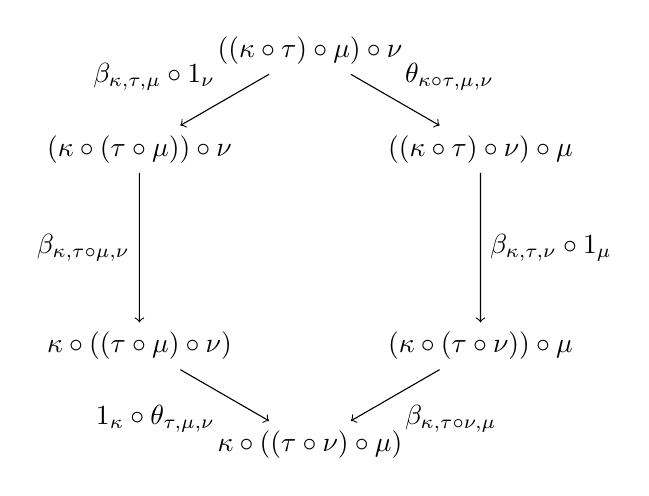
\begin{tikzpicture}[scale=2.5]
    \node (P1) at (0,1) {$((\kappa\circ\tau)\circ\mu)\circ\nu$};
    \node (P2) at (-0.866,0.5) {$(\kappa\circ(\tau\circ\mu))\circ\nu$};
    \node (P3) at (-0.866,-0.5) {$\kappa\circ((\tau\circ\mu)\circ\nu)$};
    \node (P4) at (0,-1) {$\kappa\circ((\tau\circ\nu)\circ\mu)$};
    \node (P5) at (0.866,0.5) {$((\kappa\circ\tau)\circ\nu)\circ\mu$} ;
    \node (P6) at (0.866,-0.5) {$(\kappa\circ(\tau\circ\nu))\circ\mu$};
    \draw[->] (P1)--(P2) node[midway,above left] {$\beta_{\kappa,\tau,\mu}\circ 1_\nu$};
    \draw[->] (P2)--(P3) node[midway,left] {$\beta_{\kappa,\tau\circ\mu,\nu}$};
    \draw[->] (P3)--(P4) node[midway,below left] {$1_\kappa \circ \theta_{\tau,\mu,\nu}$};
    \draw[->] (P1)--(P5) node[midway,above right] {$\theta_{\kappa\circ\tau,\mu,\nu}$};
    \draw[->] (P5)--(P6) node[midway,right] {$\beta_{\kappa,\tau,\nu}\circ 1_\mu$};
    \draw[->] (P6)--(P4) node[midway,below right] {$\beta_{\kappa,\tau\circ\nu,\mu}$};
\end{tikzpicture}
} \quad \ .
\end{center}}




%I knew that your generators  in your joint paper on the simple permuto- associahedron are note quite the same as in Mac Lane’s presentation, for example, if I understood correctly you have a generator σ for (X .Y) . ( U .V) ->  (X. U) . (Y.V).
%
%But i just realised that Kapranov’s generators are not the same either as in Mac Lane’s presentation, since for example  
%
%τ_{X.Y,U}   (X.Y) . U ->  (X.Y) . U 
%
%is a generator for Mac Lane but not for Kapranov, who accepts only τ_{X,Y} where X and Y are variables (or in ω in the terminology of your  paper).
%As a matter of fact, he has a dodecagon while Mac Lane has a hexagon. 
%
%I also realised that the hexagon can be understood as a definition of τ_{X.Y,U}, and the dodecagon as ensuring the naturality of this definition (the dodecagon is glueing two hexagons and a naturtality square in the middle). 
%
%I have two questions:
%
%1) Does this link between Kapranov’s implicit presentation (made explicit in your paper) and the hexagon based presentation (with more generators, but then addtional naturality conditions for the general τ) appear in print somewhere?
%
%2)  Was the exact correspondence between terms, morphisms, coherence conditions (Kapranov style) on one hand and 0-faces, 1-faces and 2-faces of Kapranov’s poset of faces  spelled out somewhere?


